\section{Introduction}

Generative recommendation has emerged as a transformative paradigm~\cite{GeneRec,hou2025generative,kuaishou_survey,li-etal-2024-large}, garnering substantial interest across both industry and academia~\cite{TIGER,Onerec-v2,OnePiece,MTGR}. This paradigm typically comprises two components: a tokenizer that maps each item into a sequence of tokens (\ie codewords from predefined codebooks~\cite{TIGER}) serving as its identifier~\cite{RPG,LETTER}, and a recommender that autoregressively predicts the next item based on the tokenized interaction history. By operating within a compact token space, such generative models circumvent the need for exhaustive candidate comparisons, thereby significantly enhancing scalability for massive item corpora~\cite{TIGER} and offering a compelling alternative to the traditional cascaded retrieve-and-rank framework~\cite{StreamingVQ,Trinity,RankMixer}.


Early studies in generative recommendation typically decouples the tokenizer from the recommender, optimizing them in a staged pipeline: the tokenizer is first pre-trained to generate static item identifiers, which then remain frozen during the subsequent training of the recommender~\cite{EAGER,SEATER,TIGER,LETTER,DiscRec,LC-Rec}. However, this unidirectional formulation renders the tokenizer agnostic to downstream recommendation objectives, resulting in rigid identifiers that cannot adapt to the evolving recommendation context~\cite{ETEGRec}. To address this limitation, recent studies have introduced alternating optimization strategies augmented with auxiliary losses, enabling partial coordination between the tokenizer and the recommender~\cite{BLOGER,IDGenRec,ETEGRec}. Nevertheless, due to the absence of a unified high-level objective, this epoch-wise alternation leaves the two components asynchronously updated, preventing their full alignment through genuine end-to-end joint optimization.

\begin{figure}[t]
  \centering
  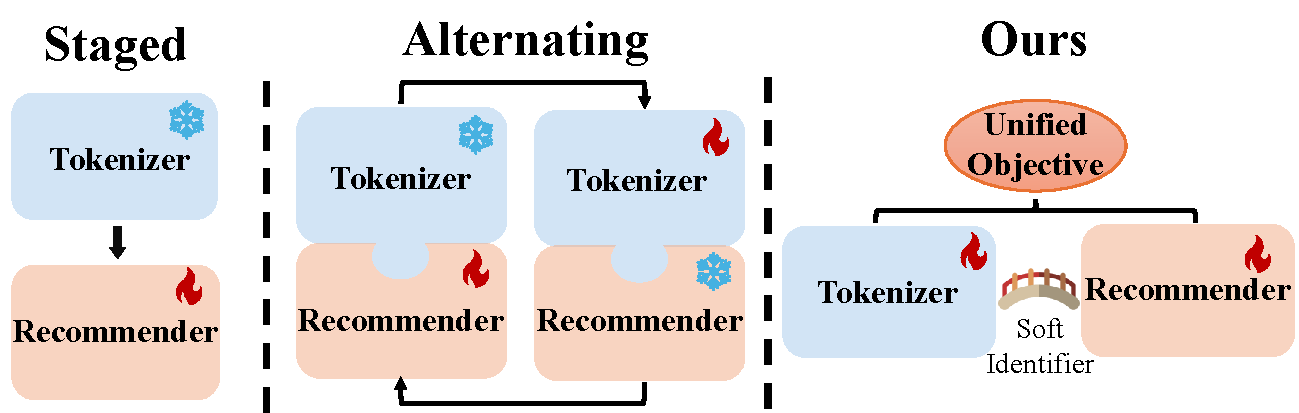
\includegraphics[width=\linewidth]{figure/paradigm_comparison.pdf}
  \caption{Comparison of generative recommendation training paradigms. Staged training separates optimization into two phases with a frozen tokenizer during recommendation training. Alternating training updates the tokenizer and recommender asynchronously without a unified objective. End-to-end joint training enables a unified gradient flow, jointly optimizing both components under a single objective.}
  \label{fig:paradigm_comparison}
\end{figure}

A natural solution to the limitations of staged and alternating training is to treat the ultimate recommendation loss as a unified objective for the tokenizer, as shown in Figure~\ref{fig:paradigm_comparison}. This can be achieved by substituting discrete codewords (\textit{hard} identifiers) with continuous assignment probabilities (\textit{soft} identifiers)~\cite{BLOGER,MMQ} as the recommender input, which introduces a \textit{differentiable} path that connects the recommendation objective to the tokenizer. On the one hand, this design unifies both components under a single objective, streamlining the training framework and facilitating seamless end-to-end alignment. On the other hand, it substantially mitigates the information loss inherent in hard quantization, enabling the model to preserve and capture richer fine-grained patterns~\cite{IBQ}.


Despite its conceptual appeal, implementing this approach introduces three significant challenges: (1) \textit{Training–Inference Discrepancy}: Continuous soft optimization during training is misaligned with discrete hard inference at test time, which leads to a substantial performance drop during deterministic item generation. (2) \textit{Item Identifier Collapse}: 
With soft identifiers, each item is associated with the entire codebook, amplifying the tendency for optimization to focus on a few dominant codewords, which results in severe codeword usage imbalance and unstable training~\cite{EdVAE,Zhu_2025_ICCV}.
(3) \textit{Collaborative Signal Deficiency}: 
While soft identifiers enhance the capture of fine-grained, token-level semantics, this microscopic focus may come at the expense of modeling coarse-grained, item-level collaborative signals~\cite{BinLLM,CoLLM,DiscRec}, which are indispensable for high-quality recommendation.

To tackle these challenges, we propose an innovative framework named \textbf{UniGRec} (Unified Generative Recommendation). First, to mitigate the training–inference discrepancy, we introduce \textit{Annealed Inference Alignment}, where the codeword assignment logits are temperature-scaled to compute probabilities during tokenization, with the temperature gradually annealed during training. This strategy enables the assignment distribution to smoothly evolve toward a sharp, near-deterministic form, thereby ensuring consistency between training and inference. Second, to address item identifier collapse, we incorporate \textit{Codeword Uniformity Regularization}, which penalizes over-concentration on dominant codewords, encouraging more diverse item identifiers and reducing codebook collisions. Third, to overcome collaborative signal deficiency, we introduce \textit{Dual Collaborative Distillation}, which distills collaborative priors from a lightweight teacher model (\eg SASRec~\cite{SASRec}), by aligning the outputs of both the tokenizer and the recommender with its pre-trained item embeddings. This mechanism explicitly reinforces coarse-grained collaborative signal extraction across items. Overall, UniGRec integrates these components into a differentiable and end-to-end training framework, enabling joint optimization of both models under a unified high-level objective --- recommendation loss. Extensive experiments on multiple real-world datasets demonstrate that UniGRec consistently outperforms existing baseline methods.


The main contributions of this work are summarized as follows:
\begin{itemize}[leftmargin=*]
\item We introduce soft identifiers in generative recommendation, allowing the ultimate recommendation loss to serve as a unified objective, and identify three key challenges arising from this design: Training–Inference Discrepancy, Item Identifier Collapse, and Collaborative Signal Deficiency.
\item We propose UniGRec, which integrates Annealed Inference Alignment, Codeword Uniformity Regularization, and Dual Collaborative Distillation to jointly optimize the tokenizer and recommender in a differentiable, end-to-end training framework.
\item We conduct extensive experiments on multiple real-world datasets, demonstrating the effectiveness of UniGRec.
\end{itemize}